
\documentclass[journal]{IEEEtran}

\usepackage[utf8]{inputenc}
\usepackage[english]{babel}
\usepackage{graphicx}

\usepackage{amsmath, amsthm, amssymb, amsfonts}
% \usepackage{algorithm}
% \usepackage{algpseudocode}
% \usepackage{minted}
\usepackage{booktabs}
\usepackage[colorlinks=true, linkcolor=red, urlcolor=cyan, citecolor=red]{hyperref}

\usepackage[numbers]{natbib}
% \setcitestyle{authoryear,open={[},close={]}} %Citation-related commands

% todo notes
\usepackage{xcolor}
\newcommand{\todo}[1]{{\color{orange} \textbf{[TODO: {#1}]}}}

% correct bad hyphenation here
\hyphenation{op-tical net-works semi-conduc-tor}


\begin{document}
%
% paper title
% Titles are generally capitalized except for words such as a, an, and, as,
% at, but, by, for, in, nor, of, on, or, the, to and up, which are usually
% not capitalized unless they are the first or last word of the title.
% Linebreaks \\ can be used within to get better formatting as desired.
% Do not put math or special symbols in the title.
\title{Advanced Machine Learning Project\\Open Graph Benchmark}
%
%
% author names and IEEE memberships
% note positions of commas and nonbreaking spaces ( ~ ) LaTeX will not break
% a structure at a ~ so this keeps an author's name from being broken across
% two lines.
% use \thanks{} to gain access to the first footnote area
% a separate \thanks must be used for each paragraph as LaTeX2e's \thanks
% was not built to handle multiple paragraphs
%

\author{Rigo Andrea}% <-this % stops a space


% note the % following the last \IEEEmembership and also \thanks - 
% these prevent an unwanted space from occurring between the last author name
% and the end of the author line. i.e., if you had this:
% 
% \author{....lastname \thanks{...} \thanks{...} }
%                     ^------------^------------^----Do not want these spaces!
%
% a space would be appended to the last name and could cause every name on that
% line to be shifted left slightly. This is one of those "LaTeX things". For
% instance, "\textbf{A} \textbf{B}" will typeset as "A B" not "AB". To get
% "AB" then you have to do: "\textbf{A}\textbf{B}"
% \thanks is no different in this regard, so shield the last } of each \thanks
% that ends a line with a % and do not let a space in before the next \thanks.
% Spaces after \IEEEmembership other than the last one are OK (and needed) as
% you are supposed to have spaces between the names. For what it is worth,
% this is a minor point as most people would not even notice if the said evil
% space somehow managed to creep in.



% The paper headers
\markboth{Advanced Topics in Machine Learning and Optimization  @ University of Trento 2023}%
{}
% The only time the second header will appear is for the odd numbered pages
% after the title page when using the twoside option.
% 
% *** Note that you probably will NOT want to include the author's ***
% *** name in the headers of peer review papers.                   ***
% You can use \ifCLASSOPTIONpeerreview for conditional compilation here if
% you desire.




% If you want to put a publisher's ID mark on the page you can do it like
% this:
%\IEEEpubid{0000--0000/00\$00.00~\copyright~2015 IEEE}
% Remember, if you use this you must call \IEEEpubidadjcol in the second
% column for its text to clear the IEEEpubid mark.



% use for special paper notices
%\IEEEspecialpapernotice{(Invited Paper)}




% make the title area
\maketitle

% As a general rule, do not put math, special symbols or citations
% in the abstract or keywords.


% Note that keywords are not normally used for peerreview papers.
% \begin{IEEEkeywords}
% IEEE, IEEEtran, journal, \LaTeX, paper, template.
% \end{IEEEkeywords}






% For peer review papers, you can put extra information on the cover
% page as needed:
% \ifCLASSOPTIONpeerreview
% \begin{center} \bfseries EDICS Category: 3-BBND \end{center}
% \fi
%
% For peerreview papers, this IEEEtran command inserts a page break and
% creates the second title. It will be ignored for other modes.
\IEEEpeerreviewmaketitle








\section*{Abstract}
In this project several models are trained and evaluated, starting from the ones seen during the lectures on Graph Neural Networks (GNNs), on the \textit{molhiv} dataset from the Open Graph Benchmark (OGB) \cite{ogbsite, hu2020ogb} on the task of graph classification.
The best model finally undergoes the evaluation procedure indicated by OGB and is compared to the models on the OGB \textit{molhiv} leaderboard.
Section \ref{sec:prob-data} will describe the problem and the dataset used, section \ref{sec:rel-works} will give a brief overview of each of the approaches used in this work, section \ref{sec:models} will talk about the models trained, section \ref{sec:exps} will describe the experiments that were carried out and their results and finally section \ref{sec:ogb-eval} will describe OGB's evaluation procedure and show the results compared to the leaderboard.
The code is available at \url{https://github.com/andrearigo-dev/aml-open-graph-benchmark}.


\section{Problem formulation and Dataset}
\label{sec:prob-data}
The task to be solved is graph classification.
Given a graph $G=(V,E)$, where $V$ is a set of nodes and $E$ is a set of edges, the task is to assign a label to the entire graph based on nodes and edges features.
In the case of \textit{molhiv}, each graph represents a molecule and the task is to predict whether a molecule inhibits HIV virus replication or not, with binary labels.
The dataset contains 41127 graphs, with an average of 25.5 nodes and 27.5 edges per graph.
Each node is associated with a 9-dimensional feature vector and each edge with a 3-dimensional one.
Given the limited computational resources available, this dataset was chosen because it is the smallest available for the task, making training and evaluation faster and therefore making development easier.
For the \textit{molhiv} dataset, OGB dictates the use of the Receiver Operating Characteristic Area Under the Curve (ROC-AUC) as evaluation metric.
The ROC curve is a graph showing the performance of a classification model at all classification thresholds by plotting the true positive rate (recall) and the false positive rate.
The area under the ROC curve measures the two-dimensional area underneath the entire the curve, which provides an aggregate measure of performance across all possible classification thresholds.


\section{Related Works}
\label{sec:rel-works}
GNNs, specifically Convolutional Graph Neural Networks (ConvGNNs), employ a series of Graph Convolution layers.
The Graph Convolution is inspired by the convolution operation on pixels in Convolutional Neural Networks (CNNs), and given a node, it aggregates its neighbor nodes' features and combines them with the node's own features, producing a new feature representation for the node itself, which is then passed to next layer.
The sequence of Graph Convolution layers in ConvGNNs gradually refines the nodes features with their neighbors'.
ConvGNNs can also be seen as a case of Message Passing Neural Network (MPNN) \cite{gilmer2017mpnn}, a general framework that groups many GNN architectures where neighboring nodes send their features through messages that get propagated along the edges of the graph and combined with the receiving node's features.
In the case of graph classification, the features of all nodes at the last layer get pooled together in a single representation for the whole graph, which is then passed to a classifier to predict a label for the graph.
This final global pooling is often called readout, and for example it can be the average of all the transformed nodes' feature vectors.
The way the neighbor information is aggregated and used to update a node's representation, as well as the readout operation, can be defined in several different ways.
This work makes use of PyTorch Geometric (PyG) \cite{fey2019pyg}, which provides many ConvGNNs components' implementations from different papers, ready for use.
Because of the ease of use of such components thanks to the library, in this work several implementations were tested, plus a few attempts at combining different approaches.
This section will briefly introduce how the various implementations work.


\subsection{Graph Convolutional Networks}
\label{sec:gcn}
The first type of GNN used for this project are the Graph Convolutional Networks (GCNs) \cite{kipf2016gcn}.
They are based on spectral convolutions on graphs \cite{bruna2014spectralcnn}, which suffer from a high computational complexity, and propose a fast approximation of it.
GCNs define the convolution operation as:
\begin{equation}
    \mathbf{X}^{\prime} = \mathbf{\hat{D}}^{-1/2} \mathbf{\hat{A}} \mathbf{\hat{D}}^{-1/2} \mathbf{X} \mathbf{\Theta}
\end{equation}
where $\mathbf{\hat{A}} = \mathbf{A} + \mathbf{I}$ is the adjacency matrix with inserted self loops, $\mathbf{\hat{D}}$ is its diagonal matrix, $\mathbf{\Theta}$ is a learnable matrix and $\mathbf{X}$ is the nodes' features matrix.
The adjacency matrix can also contain edge weights if needed.


\subsection{Modified Graph Isomorphism Network}
\label{sec:gine}
The graph isomorphism problem asks whether two graphs are topologically identical. This is a challenging problem as no polynomial-time algorithm to solve it is known.
The Weisfeiler-Lehman (WL) \cite{weisfeiler1968wl} test of graph isomorphism is an effective and computationally efficient test that distinguishes a broad class of graphs.
\citet{xu2018gin} studied the representational power of several GNN variants and postulated that no GNN can have a higher representational power than the WL test.
They then designed the Graph Isomorphism Network (GIN), a GNN as expressive as the test.
\cite{hu2019gine} then proposed a modified version of GIN, that PyG calls GINE, that supports edge features.
The convolution operator is defined as:
\begin{equation}
    \mathbf{x}^{\prime}_i = h_{\mathbf{\Theta}} \left( (1 + \epsilon) \cdot \mathbf{x}_i + \sum_{j \in \mathcal{N}(i)} \mathrm{ReLU} ( \mathbf{x}_j + \mathbf{e}_{j,i} ) \right)
\end{equation}
where $h_{\mathbf{\Theta}}$ is a neural network, i.e. a Multi Layer Perceptron (MLP), $\mathbf{x}_i$ are node features and $\mathbf{e}_{j,i}$ are edge features.


\subsection{SAGE: SAmple and aggreGatE}
\label{sec:sage}
\citet{hamilton2017sage} proposed a general framework called GraphSAGE (SAmple and aggreGatE), or simply SAGE.
At at each iteration, SAGE aggregates information from the local neighbors of node $v$ at layer $k$:
\begin{equation}
    \mathbf{h}_{\mathcal{N}(v)}^{k}\leftarrow\operatorname{AGGREGATE}_{k}(\{\mathbf{h}_{u}^{k-1},\forall u\in\mathcal{N}(v)\})
\end{equation}
where $\mathcal{N}(v)$ is the local node $v$ neighborhood, $\mathbf{h}_{\mathcal{N}(v)}^{k}$ are the neighbors aggregated features at layer $k$ and $\mathbf{h}_{u}^{k-1}$ is the feature vector of a neighbor node $u$ at the previous layer $k-1$.
Then the aggregated information is combined to the node own features:
\begin{equation}
    \mathbf{h}_v^k\leftarrow\sigma\left(\mathbf{W}^k\cdot\operatorname{CONCAT}(\mathbf{h}_v^{k-1},\mathbf{h}_{\mathcal{N}(v)}^k)\right)
\end{equation}
where $\mathbf{W}^k$ is a learnable weight matrix and $\sigma$ is a non linearity.
Each layer aggregates information from each node local neighbors, and as this process iterates, nodes incrementally gain more and more information from further reaches of the graph.
The $\mathrm{AGGREGATE}$ operator can be defined in different ways.
In the paper \cite{hamilton2017sage} the authors implement the mean aggregator, which simply takes the elementwise mean of the neighbors' feature vectors, a Long Short Term Memory Network (LSTM) and finally the \textit{pooling} aggregator, which PyG simply calls \textit{max}, where each neighbor’s vector is independently fed through a fully-connected neural network, then all the transformed vectors are fed to a max-pooling operation.


\subsection{Graph Attention Networks v2}
\label{sec:gatv2}
\citet{velickovic2017gat} proposed the Graph Attention Network (GAT), which uses self attention to allow each node to attend to each other nodes in its neighborhood.
Given a query node $i$, the graph attention layer computes attention scores between the node and its neighbors, including $i$ itself, then combines the neighbors information using the attention scores as weights to give more importance to the more relevant neighbors for $i$.
Later, \citet{brody2021gatv2} discovered that the attention mechanism employed by GAT has some limitations, as it can't model situations where different keys have different relevance to different queries.
So, they proposed a slightly modified GAT, GATv2, that solves this issue and makes GAT more expressive.
The nodes' features are combined as follows:
\begin{equation}
    \mathbf{x}^{\prime}_i = \alpha_{i,i}\mathbf{\Theta}\mathbf{x}_{i} + \sum_{j \in \mathcal{N}(i)} \alpha_{i,j}\mathbf{\Theta}\mathbf{x}_{j}
\end{equation}
where $\alpha_{i,j}$ is the attention score between nodes $i$ and $j$, $\mathbf{x}_{i}$ are node $i$ features, $\mathbf{\Theta}$ is a learned matrix that transforms the features and $\mathcal{N}(i)$ is the neighborhood.
The attention coefficients are computed as follows:
\begin{equation}
    \alpha_{i,j} = \frac{\exp\left(\mathbf{a}^{\top}\mathrm{LeakyReLU}\left(\mathbf{\Theta} [\mathbf{x}_i \, \Vert \, \mathbf{x}_j \, \Vert \, \mathbf{e}_{i,j}] \right)\right)} {\sum_{k \in \mathcal{N}(i) \cup \{ i \}} \exp\left(\mathbf{a}^{\top}\mathrm{LeakyReLU}\left(\mathbf{\Theta} [\mathbf{x}_i \, \Vert \, \mathbf{x}_k \, \Vert \, \mathbf{e}_{i,k}] \right)\right)}
\end{equation}
where $\mathbf{e}_{i,j}$ are multidimensional edge features.
GATv2 also supports multi-head attention.


\subsection{Attentional Aggregation}
\label{sec:attnaggr}
\citet{li2019attnaggr} proposed an Attentional Aggregator, which aggregates nodes features using a sum weighted by attention scores:
\begin{equation}
    \mathbf{r}_i = \sum_{n=1}^{N_i} \mathrm{softmax} \left(h_{\mathrm{gate}} ( \mathbf{x}_n ) \right) \cdot h_{\mathbf{\Theta}} ( \mathbf{x}_n )
\end{equation}
where $h_{\mathrm{gate}}$ and $h_{\mathbf{\Theta}}$ are two neural networks, for example MLPs, the former computes the attention scores and the latter transforms the features to the desired output dimension before combining them to the scores.


\subsection{Differentiable Pooling}
\label{sec:diffpool}
All GNNs seen above progressively refine node representations using neighbors information.
However they don't learn any hierarchical structure between nodes, nor they use any pooling operation, both things that proved effective in CNNs to learn complex patterns.
\citet{ying2018diffpool} proposed DiffPool, a differentiable graph pooling module that can generate hierarchical graph representations.
DiffPool learns a differentiable soft cluster assignment for nodes at each layer of a deep GNN, mapping nodes to a set of clusters, which then form the coarsened input for the next GNN layer.
Given the soft cluster assignment matrix $\mathbf{S}$, the nodes' features $\mathbf{X}$ and the graph adjacency matrix $\mathbf{A}$, a DiffPool layer coarsens the input graph, generating a new coarsened adjacency matrix $\mathbf{A}^{\prime}$ and a new matrix of embeddings $\mathbf{X}^{\prime}$ for each of the nodes/clusters in this coarsened graph by computing the weighted combination of cluster members:
\begin{align}
    \begin{aligned}
        \mathbf{X}^{\prime} &= {\operatorname{softmax}(\mathbf{S})}^{\top} \cdot \mathbf{X}\\
        \mathbf{A}^{\prime} &= {\operatorname{softmax}(\mathbf{S})}^{\top} \cdot \mathbf{A} \cdot \operatorname{softmax}(\mathbf{S})
    \end{aligned}
\end{align}
The soft clustering matrix and node embeddings can be computed by any GNN module.
Learning to cluster nodes using the graph label as the only source of supervision can be hard since the signal is very indirect.
So the authors use two side objectives:
\begin{align}
    \begin{aligned}
        \mathcal{L}_{LP} &= {\| \mathbf{A} - \operatorname{softmax}(\mathbf{S}) {\operatorname{softmax}(\mathbf{S})}^{\top} \|}_F,\\
        \mathcal{L}_E &= \frac{1}{N} \sum_{n=1}^N H(\mathbf{S}_n)
    \end{aligned}
\end{align}
where $\mathcal{L}_{LP}$ is a link prediction loss encouraging nearby nodes to be pooled together, and $\mathcal{L}_E$ is the cluster entropy, encouraging hard assignments.


\section{Models}
\label{sec:models}
This work first designs a base GNN, inspired by the PyG example code, then all following models are variations of it.
The GNN architecture is illustrated in figure \ref{fig:gnn-scheme} and uses an Atom Encoder, which is a node encoder provided by OGB, followed by a block composed of a Graph Convolution layer, a Batch Norm \cite{ioffe2015batchnorm} layer followed by the ReLU non-linearity, a Dropout layer with $p=0.5$ and a residual connection that skips all the mentioned layers and propagates the signal as-is from the previous block or the Atom Encoder.
Based on the parameter \textit{layers} that determines the number of layers in the network, the block is repeated.
Finally a readout operation is performed, combining all node embeddings into a single graph representation, which is then classified by being fed to a Linear layer and transformed into a probability with the Sigmoid function.
Additionally, an $\operatorname{MLP}$ and $\operatorname{MLP}_{gate}$ networks are defined, which are necessary for some models.
The former, is composed of a Linear layer doubling the hidden channels, a Batch Norm layer, ReLU activation function and another Linear layer that decreases the hidden channels back to the original dimension.
The latter, has the same architecture, but decreases the hidden channels to 1 with the last Linear layer, and finally normalizes the output in the $[-1,1]$ range using an hyperbolic tangent (Tanh).
From now on, when referring to either of the two networks, it means a network with same architecture, not the same network as in the same trained weights.

\begin{figure}
    \centering
    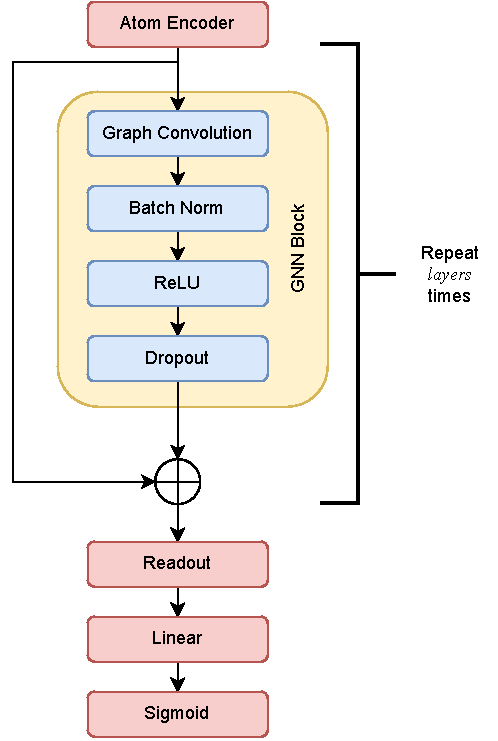
\includegraphics[width=0.48\textwidth]{figures/gnn-scheme.drawio.pdf}
    \caption{Base GNN scheme}
    \label{fig:gnn-scheme}
\end{figure}

The models used in this work, deriving from the base one, are the following:
\begin{enumerate}
    \item GCN: This model is simply the base GNN, using GCN convolutions \cite{kipf2016gcn} (Section \ref{sec:gcn}) as Graph Convolution block.
    \item EdgeGCN: The dataset comes with 3-dimensional edge features but GCN convolutions only support scalar weights, all set to 1 by default. So, in an attempt to make the GCN model aware of edge features, the edges' feature vectors are encoded by a Bond Encoder, which is OGB's provided edge encoder, and then fed to an $\operatorname{MLP}_{gate}$ that predicts a weight for the edge. The weight is than translated by two, bringing it into the $[1,3]$ range:
    \begin{equation}
        \mathbf{w}_{i,j} = \operatorname{MLP}_{gate}(\operatorname{BondEnc}(\mathbf{e}_{i,j})) + 2
    \end{equation}
    where $\mathbf{w}_{i,j}$ is the resulting edge weight, $\mathbf{e}_{i,j}$ are the edge's features, and $\operatorname{BondEnc}$ is the Bond Encoder.
    \item GINE: Base GNN using GINE convolutions \cite{hu2019gine} (Section \ref{sec:gine}), with $h_{\mathbf{\Theta}} = \operatorname{MLP}$ to transform features. It also uses a Bond Encoder for edge features.
    \item GAT: Base GNN using GATv2 convolutions \cite{brody2021gatv2} (Section \ref{sec:gatv2}). Again, a Bond Encoder is used. The model is trained using 8 attention heads. Keep in mind however, that here for simplicity the model uses GNN Blocks with GATv2 convolutions, while in the original paper the authors only used GATv2 layers, with no Batch Norm or Dropout.
    \item SAGE: Base GNN using SAGE convolutions \cite{hamilton2017sage} (Section \ref{sec:sage}).
    \item DiffPool: Here, a DiffPool layer \cite{ying2018diffpool} (Section \ref{sec:diffpool}) is placed every two GNN Blocks, except for the last layer. For example, for a 6 blocks network, there would be 3 DiffPool layers, and one would be after last GNN Block. This last DiffPool layer is not placed. As in the original paper, every GNN Block uses SAGE convolutions, and the DiffPool layers also use SAGE convolutions for transforming node features and for predicting the soft cluster assignments.
\end{enumerate}


\section{Experiments}
\label{sec:exps}
All the models have a final readout step, which uses an aggregator to combine all nodes features.
SAGE convolutions aggregate features using an arbitrary aggregator function.
The DiffPool model uses SAGE convolutions both in the GNN Blocks and in the pooling layers, therefore it also requires an aggregator function.
Each aggregator in each model can either be a \textit{mean} aggregator or a \textit{max} aggregator, which simply takes the maximum of the features, except in the case of SAGE in which \textit{max} refers to the \textit{pooling} aggregator (Section \ref{sec:sage}).
Additionally, an Attentional Aggregator \cite{li2019attnaggr} (Section \ref{sec:attnaggr}) can be used in any of the above, adding an attentional component to models that wouldn't have it otherwise.
Hence here all the architectures described in previous sections are tested using different aggregators in the readout step, in the graph convolutions and in the pooling layers in order to explore which aggregators and models work best.
In the case of the Attentional Aggregator, $h_{\mathrm{gate}} = \operatorname{MLP}_{gate}$ and $h_{\mathbf{\Theta}} = \operatorname{MLP}$ are used to compute the attention scores and transform features.
All models were trained with the following parameters: batch size 64, 200 epochs, learning rate 0.001, 300 hidden channels for all the Graph Convolutions and 6 layers.
The number of layers represents the number of GNN Blocks. In the case of DiffPool models, in addition to the 6 GNN Blocks there is a DiffPool layer every two of them.
DiffPool layers also require an additional parameter, which is called \textit{ReduceTo} in the code, that represents the number of clusters to assign nodes to, expressed as a percentage of number of clusters already present before applying the layer, or the number of nodes in the graph if no other pooling layer was applied before.
Suppose a DiffPool layer groups nodes into 20 clusters, the next DiffPool must reduce the number of clusters to learn a hierarchical structure.
So it will reduce the number of cluster to some percentage of the previous number.
This parameter is set to 25\%. In this example, the second DiffPool layer would cluster nodes to $20 \cdot 0.25=5$ clusters.
One DiffPool model with a more aggressive clustering was also trained, with \textit{ReduceTo} set to 50\%.
At every epoch the models were evaluated on the validation set, and at the end of the training the best epochs were taken for comparison.

Table \ref{tab:eval-res} shows the results, and shows the trained model along with which type of aggregation was used by Graph Convolutions in the GNN Block and in the pooling layers as well as the readout. When the readout is set to \textit{Pooling}, a DiffPool layer is used to group all nodes into a single cluster.
The table also highlights the best model, which was DiffPool using \textit{max} aggregation in the Graph Convolutions of the GNN Block, in the pooling layers and as readout.

The hyperparameters for the best model are then tuned using a grid search.
The grid search trains and evaluates the model with all possible hyperparameters combinations from a predefined set of values and outputs the best configuration.
Due to the computational resources available the search space is quite limited. Table \ref{tab:hyper-search-space} shows the possible parameters values.

\begin{table}[ht]
\centering
\begin{tabular}{@{}cc@{}}
\toprule
\textbf{Hyperparameter} & \textbf{Values} \\ \midrule
Batch size              & 32, 64          \\
Number of layers        & 6, 8, 10        \\
Learning rate           & 0.001           \\
Hidden channels         & 300             \\
Epochs                  & 200             \\ \bottomrule\\
\end{tabular}
\caption{Hyperparameters search space}
\label{tab:hyper-search-space}
\end{table}

\noindent The best configuration turned out to be initial one, described above.


\section{OGB Evaluation}
\label{sec:ogb-eval}
The best model with the best configuration was then evaluated following OGB instructions: use OGB's provided evaluators to train and validate the model on both the test and validation set 10 times with 10 different random seeds, then report the average and standard deviation.
The results are shown in table \ref{tab:ogb-eval-res}.
For comparison to the \textit{molhiv} dataset leaderborad we will use the scores rounded to four decimals: 0.7712 \textpm 0.0130 for test and 0.8548 \textpm 0.0087 for validation.
If it were to be submitted to the leaderboard at the time of writing this report, DiffPool would take the 27th place, as its test ROC-AUC is better than GIN+Virtual Node \cite{xu2018gin} but worse than Efficient Graph Convolution-Single (EGC-S) \cite{tailor2021egc}.
The former is a GIN where a virtual node connected to all the other nodes was added to the graph at the last layer. The neighborhood of the virtual node is the entire graph, so a GIN convolution will combine all nodes embeddings into a single final one before classification.
The latter is an MPNN where messages don't depend on the target node, but only on the source, which also aims to be more computationally efficient than commonly used GNNs.


\section{Conclusion}
Given the relative simplicity of the model and the scarce computational resources making deeper and larger architectures unfeasible, the 27th place on 33 is not a great achievement but I think it's enough for a small university project.
For comparison, among the top of the leaderbaord there are much more complex and larger models, such as Graphormer \cite{ying2021graphormer}, a Transformer \cite{vaswani2017transformer} adapted to work on graph data and the best model, Pooling Architecture Search (PAS) \cite{Wei2021pas}, which uses Neural Architecture Search to search for an effective architecture for graph classification.


% \nocite*
% \bibliographystyle{ieeetr}
% \bibliographystyle{plainnat}
\bibliographystyle{apalike}
\bibliography{bib}


\onecolumn
\begin{table}[ht]
\centering
\begin{tabular}{@{}ccccc@{}}
\toprule
\textbf{Model}          & \textbf{Readout}      & \textbf{Aggregation} & \textbf{Pooling Aggregation} & \textbf{Validation ROC-AUC} \\ \midrule
GINE     & Mean        & -           & -           & 0.7243 \\
GCN      & Mean        & -           & -           & 0.8202 \\
GCN      & Attentional & -           & -           & 0.8078 \\
EdgeGCN  & Mean        & -           & -           & 0.8243 \\
EdgeGCN  & Attentional & -           & -           & 0.8179 \\
GAT      & Mean        & -           & -           & 0.8257 \\
SAGE     & Mean        & Mean        & -           & 0.8354 \\
SAGE     & Max         & Max         & -           & 0.8415 \\
SAGE     & Mean        & Max         & -           & 0.8446 \\
SAGE     & Attentional & Max         & -           & 0.8483 \\
SAGE     & Max         & Attentional & -           & 0.8216 \\
SAGE     & Attentional & Attentional & -           & 0.8532 \\
DiffPool & Mean        & Mean        & Mean        & 0.8382 \\
DiffPool & Mean        & Max         & Attentional & 0.8471 \\
DiffPool                & Pooling (Attentional) & Attentional          & Attentional                  & 0.8423                      \\
DiffPool, \textit{ReduceTo} 50\% & Attentional           & Max                  & Max                          & 0.8562                      \\
DiffPool & Attentional & Max         & Max         & 0.8594 \\
\textbf{DiffPool}       & \textbf{Max}          & \textbf{Max}         & \textbf{Max}                 & \textbf{0.8597}             \\ \bottomrule\\
\end{tabular}
\caption{Evaluation results}
\label{tab:eval-res}
\end{table}

\begin{table}[ht]
\centering
\begin{tabular}{@{}ccc@{}}
\toprule
\textbf{Seed}      & \textbf{Test ROC-AUC}                              & \textbf{Validation ROC-AUC}                        \\ \midrule
0 & 0.7599528766488346 & 0.8641148805618286 \\
1 & 0.7678228625504547 & 0.8619133234024048 \\
2 & 0.774825701539234  & 0.8579328060150146 \\
3 & 0.7743486741729273 & 0.8488297462463379 \\
4 & 0.7651885899689064 & 0.834518313407898  \\
5 & 0.7737577009984743 & 0.8518151044845581 \\
6 & 0.7913246683018212 & 0.8569315671920776 \\
7 & 0.7526603449274801 & 0.8628073930740356 \\
8 & 0.7921377392379151 & 0.8527275919914246 \\
9 & 0.7599007319569709 & 0.8560864925384521 \\
\textbf{AVG \textpm STD} & \textbf{0.7711919546127319 \textpm 0.012988988310098648} & \textbf{0.8547677993774414 \textpm 0.008677446283400059} \\ \bottomrule\\
\end{tabular}
\caption{DiffPool OGB evaluation results}
\label{tab:ogb-eval-res}
\end{table}

% Can use something like this to put references on a page
% by themselves when using endfloat and the captionsoff option.
\ifCLASSOPTIONcaptionsoff
  \newpage
\fi




\end{document}


